\documentclass[11pt]{article}
\usepackage{amsmath, amssymb, enumitem, fancyhdr, graphicx, libertine, nth,
  pgfplots, tikz, xcolor}
\pgfplotsset{compat=1.11}
\usepackage[margin=1in]{geometry}
\usepackage[libertine]{newtxmath}
\pagestyle{fancy}
\definecolor{solution-color}{HTML}{000080}
\chead{\emph{EC201 -- Final Exam Solutions -- August \nth{9}}}

% Define new topic command
\newcommand{\topic}[1]{\medskip\begin{center}\large\textsc{#1}\normalsize
  \end{center}}
% Define question counter:
\newcounter{question}[section]
\newcommand{\question}[1]{\refstepcounter{question}
  \subsubsection*{Question~\thequestion~-- #1}}

% Subquestions are enumerate with letters
\newenvironment{subquestions}{
  \begin{enumerate}[label=(\roman*)]}{\end{enumerate}}

\begin{document}
\question{Preferences (10 Points, 13.5 minutes)}
The following parts (i), (ii) and (iii) of this question are \emph{unrelated}.
Consider each separately. Each bundle $\left( x_1,x_2 \right)$ are different amounts of the same two goods, Good 1 and Good 2.
\begin{subquestions}
\item \textbf{(3 Points)} Mary says she strictly prefers $\left( 2,3 \right)$ to $\left( 1,3 \right)$. Mary also says she strictly prefers $\left( 1,3 \right)$ to $\left( 3,1 \right)$. So $\left( 2,3 \right)\succ\left( 1,3 \right)$ and $\left( 1,3\right)\succ \left( 3,1 \right)$.
    \begin{itemize}
      \item If Mary prefers $\left( 3,1\right)$ to $\left( 2,3 \right)$, then what common assumption of preferences does he violate?

        \textcolor{solution-color}{By transitivity, Mary should prefer $\left( 2,3 \right)$ to $\left( 3,1 \right)$. Therefore she violates transitivity.}
    \end{itemize}
  \item \textbf{(3 Points)} John says he strictly prefers $\left( 1,2 \right)$ to $\left( 100,1 \right)$. This means that $\left( 1,2 \right)\succ \left( 100,1 \right)$.
    \begin{itemize}
      \item Do John's preferences violate monotonicity? Why or why not?

        \textcolor{solution-color}{No. $\left( 100,1 \right)$ does not have at least as much of \emph{both} goods as $\left( 1,2 \right)$. Therefore this preference relation does not violate monotonicity.}
    \end{itemize}
  \item \textbf{(4 Points)} Emma's preferences satisfy completeness, transitivity, reflexivity, monotonicity and convexity. Emma says she is indifferent between the bundles $\left( 1,9 \right)$ and $\left( 9,1 \right)$. This means that $\left( 1,9 \right)\sim \left( 9,1 \right)$.
    \begin{itemize}
      \item If you gave Emma the choice between $\left( 6,6 \right)$ and $\left( 1,9 \right)$, which would she choose? Assume both are affordable. Carefully explain your reasoning outlining which properties of Emma's preferences (completeness, transitivity, reflexivity and monotonicity) you need to make your conclusion (there may be more than one).

        \textcolor{solution-color}{Since $\left( 1,9 \right)\sim\left( 9,1 \right)$, convexity tell us that $\left( 5,5 \right)\succeq\left( 1,9 \right)$. By monotonicity, $\left( 6,6 \right)\succ \left( 5,5 \right)$. Therefore by transitivity $\left( 6,6 \right)\succ \left( 1,9 \right)$.}
    \end{itemize}
\end{subquestions}

\question{Choice, Demand and Elasticities (10 Points, 13.5 minutes)}
Your utility function for goods 1 and 2 is:
\[
  u\left( x_1,x_2 \right)=x_1^{\frac{1}{2}} + \frac{1}{2}x_2
\]
\begin{subquestions}
\item \textbf{(4 Points)} Show that the demand function for good 1 is $x_1\left( p_1,p_2,m \right)=\frac{p_2^2}{p_1^2}$ and the demand function for good 2 is $x_2\left( p_1,p_2,m \right)=\frac{m}{p_2}-\frac{p_2}{p_1}$. Show your work for each step.

  \textcolor{solution-color}{
    First we use the $\frac{MU_1}{MU_2}=\frac{p_1}{p_2}$ optimality condition:
    \[\frac{\frac{1}{2}x_1^{-\frac{1}{2}}}{\frac{1}{2}}=\frac{p_1}{p_2}
      \;\;\;\Longrightarrow\;\;\;
    x_1^{-\frac{1}{2}}=\frac{p_1}{p_2}
      \;\;\;\Longrightarrow\;\;\;
    x_1^{\frac{1}{2}}=\frac{p_2}{p_1}
      \;\;\;\Longrightarrow\;\;\;
    x_1=\frac{p^2_2}{p^2_1}
    \]
    Using this in the budget line:
    \begin{align*}
      p_1x_1+p_2x_2&=m\\
      p_1\frac{p^2_2}{p^2_1}+p_2x_2&=m\\
      \frac{p^2_2}{p_1}+p_2x_2&=m\\
      p_2x_2&=m-\frac{p^2_2}{p_1}\\
      x_2&=\frac{m}{p_2}-\frac{p^2}{p_1}
    \end{align*}
  }
\item \textbf{(4 Points)} What is the own-price elasticity of demand for good 1? Is it elastic, inelastic or unit elastic?

  \textcolor{solution-color}{
    Demand for good 1 can be rewritten as $x_1\left( p_1,p_2,m \right)=p_2^2p_1^{-2}$ so the derivative with respect to $p_1$ is $-2p_2^2p_1^{-3}=-2\frac{p_2^2}{p_1^3}$. The elasticity is then:
    \[
      \varepsilon_1=\frac{\partial x_1\left( p_1,p_2,m \right)}{\partial p_1}\frac{p_1}{x_{1}\left( p_1,p_2,m \right)}=\left( -2\frac{p_2^2}{p_1^3}\right)\frac{p_1}{\left( \frac{p_2^2}{p_1^2} \right)}=-2
    \]
    Since $\left| \varepsilon_1 \right|=2>1$, it is elastic.
   }
  \item \textbf{(1 Point)} Are the two goods substitutes or complements?

  \textcolor{solution-color}{
    If the price of the other good increases, demand for the good increases. Therefore they are substitutes.
  }
  \item \textbf{(1 Point)} Is good 2 normal or inferior (or neither)?

  \textcolor{solution-color}{
    If income increases, the demand for good 2 increases. Therefore good 2 is normal.
  }
\end{subquestions}

\question{Perfect Complements and Income and Substitution Effects (13 Points, 17.5 minutes)}
Your utility function for goods 1 and 2 is $u\left( x_1,x_2 \right)=\min\left\{ x_1,x_2 \right\}$.
\begin{subquestions}
\item \textbf{(3 Points)} Find the demand functions for goods 1 and 2. Show your reasoning.

  \textcolor{solution-color}{
    At the optimum choice $x_1=x_2$. This is because if you buy unequal amounts of the goods you don't get any extra utility from the good you have more of and you use up your income on it. Using this in the budget line:
    \begin{align*}
      p_1x_1 + p_2x_1 &= m \\
      x_1\left( p_1+p_2 \right) &= m \\
      x_1 &= \frac{m}{p_1+p_2} \\
    \end{align*}
    So $x_1\left( p_1,p_2,m \right)=x_2\left( p_1,p_2,m \right)=\frac{m}{p_1+p+2}$.
  }
  \item \textbf{(1 Point)} The prices for both goods 1 and 2 are currently \$2. You have \$120 to spend. How much of each good will you buy?

  \textcolor{solution-color}{
    You will buy $\frac{120}{2+2}=\frac{120}{4}=30$ of each good.
  }
  \item \textbf{(1 Point)} The price of good 1 decreases to \$1. The price of good 2 is still \$2 and you still have \$120 to spend. How much of each good will you buy?

  \textcolor{solution-color}{
    You will buy $\frac{120}{1+2}=\frac{120}{3}=40$ of each good.
  }
  \item \textbf{(3 Points)} Show parts (ii) and (iii) on a graph. Show the original budget line, the new budget line, the optimal bundles and the indifference curves associated with the optimal bundles. Label all axes and points.
    \begin{center}
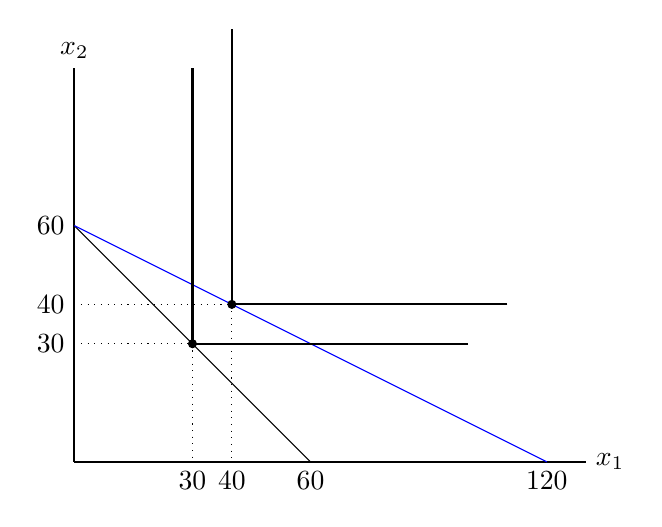
\begin{tikzpicture}[scale=.05]
    \draw [thick] (0,0) -- (130,0);
    \draw [thick] (0,0) -- (0,100);
    \node [right] at (130,0) {$x_1$};
    \node [above] at (0,100) {$x_2$};
    \draw (60,0)--(0,60);
    \draw[blue] (120,0)--(0,60);
    \node [left] at (0,60) {60};
    \node [left] at (0,30) {30};
    \node [left] at (0,40) {40};
    \node [below] at (60,0) {60};
    \node [below] at (30,0) {30};
    \node [below] at (40,0) {40};
    \node [below] at (120,0) {120};
    \draw[fill] (30,30) circle [radius=1];
    \draw[fill] (40,40) circle [radius=1];
    \draw[thick] (100,30)--(30,30);
    \draw[thick] (30,30)--(30,100);
    \draw[thick] (110,40)--(40,40);
    \draw[thick] (40,40)--(40,110);
    \draw[dotted] (30, 30) -- (30, 0);
    \draw[dotted] (0, 30) -- (30, 30);
    \draw[dotted] (40, 40) -- (40, 0);
    \draw[dotted] (0, 40) -- (40, 40);
  \end{tikzpicture}
    \end{center}

  \item \textbf{(3 Points)} Decompose the income and substitution effects of the change in price of good 1 on the demand for good 1. Draw your graph in part (iv) again but add the compensating budget line that brings you back to your original purchasing power.
    \begin{center}
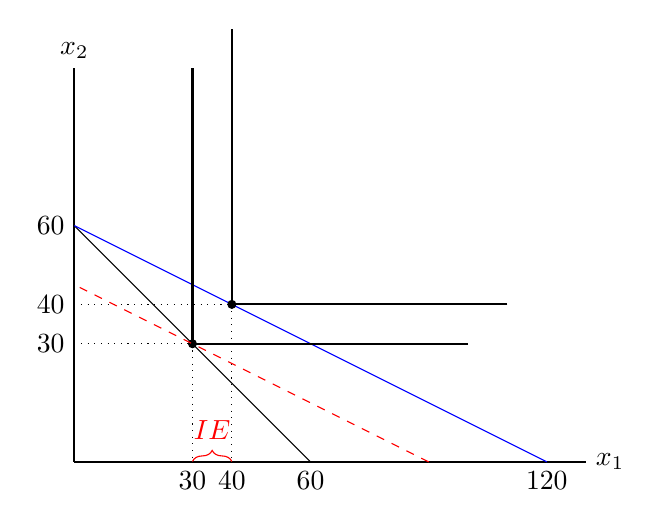
\begin{tikzpicture}[scale=.05]
    \draw [thick] (0,0) -- (130,0);
    \draw [thick] (0,0) -- (0,100);
    \node [right] at (130,0) {$x_1$};
    \node [above] at (0,100) {$x_2$};
    \draw (60,0)--(0,60);
    \draw[blue] (120,0)--(0,60);
    \node [left] at (0,60) {60};
    \node [left] at (0,30) {30};
    \node [left] at (0,40) {40};
    \node [below] at (60,0) {60};
    \node [below] at (30,0) {30};
    \node [below] at (40,0) {40};
    \node [below] at (120,0) {120};
    \draw[fill] (30,30) circle [radius=1];
    \draw[fill] (40,40) circle [radius=1];
    \draw[thick] (100,30)--(30,30);
    \draw[thick] (30,30)--(30,100);
    \draw[thick] (110,40)--(40,40);
    \draw[thick] (40,40)--(40,110);
    \draw[dotted] (30, 30) -- (30, 0);
    \draw[dotted] (0, 30) -- (30, 30);
    \draw[dotted] (40, 40) -- (40, 0);
    \draw[dotted] (0, 40) -- (40, 40);
    \draw[dashed,red] (90,0)--(0,45);
    \draw [red,decorate,decoration={brace,amplitude=4pt},xshift=0pt,yshift=3pt]
    (30,0) -- (40,0) node [red,midway,yshift=.4cm] {$IE$};
  \end{tikzpicture}
    \end{center}
    \textcolor{solution-color}{
      Note that the income effect $IE$ is highlighted, yet wasn't required for full points.
    }
  \item \textbf{(2 Point)} What are the values of the income and substitution effects for your demand for good 1?

    \textcolor{solution-color}{
      The substitution effect is zero and the income effect is 10. On the compensating budget line you would not change your optimal choice as it would involve consuming more of good 1 and less of good 2 which is worse.
    }
\end{subquestions}

\question{Intertemporal Choice (8 Points, 11 minutes)}
You live for two periods. In the first period you do not earn any money ($m_1=0$). In the second period you earn $m_2=110$. Your lifetime utility function is:
\[u\left( c_1,c_2 \right)=c_1c_2
\]$c_1$ is your consumption in period 1 and $c_2$ is your consumption in period 2. There is no inflation. There is a bank with which you can borrow and lend at an interest rate of $r=0.1$.
\begin{itemize}
  \item How much will you consume in period 1 and how much will you consume in period 2 in order to maximize your lifetime utility?
\end{itemize}
\textcolor{solution-color}{
  The optimal choice in intertemporal choice problems is where $MRS=-\left( 1+r \right)$. The $MRS$ here is simply $MRS=-\frac{c_2}{c_1}$. Therefore $c_2=\left( 1+r \right)c_1$. Using this in the budget line:
  \[m_1+ \frac{m_2}{1+r}=c_1 + \frac{c_2}{1+r}
    \;\;\;\Longrightarrow \;\;\;
    0 + \frac{110}{1.1}=c_1 + \frac{\left( 1+r \right)c_1}{1+r}
    \;\;\;\Longrightarrow \;\;\;
    100=2c_1
    \;\;\;\Longrightarrow \;\;\;
    c_1=50
  \]
  Therefore $c_2=\left( 1+r \right)c_1=1.1\times 50 = 55$. So the optimal consumption plan is $\left( c_1,c_2 \right)=\left( 50,55 \right)$.
}


\question{Cost Curves, Firm Supply and Industry Supply (14 Points, 19 minutes)}
The cost function for each firm in a \emph{perfectly competitive} industry is given by:
\[
  c\left( q \right)=q^2+1
\]
All firms have the same cost function. The market demand function for the good sold in this industry is:
\[
  D\left( p \right)=100-10p
\]
There are currently 30 firms in the industry.
\begin{subquestions}
  \item \textbf{(1 Point)} What is each firm's average cost function?
  \textcolor{solution-color}{
  \[ AC\left( q \right)=\frac{q^2+1}{q}=q+\frac{1}{q}\]
  }
  \item \textbf{(1 Point)} What is each firm's marginal cost function?
  \textcolor{solution-color}{
    \[ MC\left( q \right)=\frac{dc\left( q \right)}{dq}=2q\]
  }
  \item \textbf{(2 Point)} What is each firm's supply curve?
  \textcolor{solution-color}{
    \[ p=MC\left( q^\star \right)
    \;\;\;\Longrightarrow\;\;\;
    p=2q^\star
    \;\;\;\Longrightarrow\;\;\;
    q^\star = \frac{p}{2}
    \;\;\;\Longrightarrow\;\;\;
    S_i\left( p \right) = \frac{p}{2}
  \]
  }
  \item \textbf{(1 Point)} What is the industry supply curve?
  \textcolor{solution-color}{
    \[ S\left( p \right)= 30 \times S_i\left( p \right)=15p\]
  }
  \item \textbf{(2 Points)} What is the equilibrium market price?
  \textcolor{solution-color}{
    \[ D\left( p \right)=S\left( p \right)
    \;\;\;\Longrightarrow\;\;\;
    100-10p = 15p
    \;\;\;\Longrightarrow\;\;\;
    25p=100
    \;\;\;\Longrightarrow\;\;\;
    p=4
    \]
  }
  \item \textbf{(1 Point)} How much will each individual firm produce?

  \textcolor{solution-color}{
    Using $p=4$ in the individual firm's supply function: $S_i\left( p \right)=\frac{p}{2}=\frac{4}{2}=2$.
  }
  \item \textbf{(2 Point)} What will each firm's profits/losses be?

  \textcolor{solution-color}{
    Profits are:
    \[
      pq - q^2 - 1 = 4\times 2 - 2^2 - 1 = 3
    \]
  }
  \item \textbf{(4 Points)} How many firms will be in this industry in the long run?

  \textcolor{solution-color}{
    In the long run, profits are zero so price must equal average cost for each firm. Since marginal cost equals average cost for each firm:
    \[
      2q=q+\frac{1}{q}\;\;\;\Longrightarrow \;\;\;
      q=\frac{1}{q} \;\;\;\Longrightarrow \;\;\;
      q=1
    \]
    If each firm produces 1 unit, the marginal cost is $MC\left( q \right)=2q=2$ so the price is 2. At a price of 2, total demand is $D\left( p \right)=100-10p=100-20=80$. If the total quantity is 80 and each firm produces 1 unit, there are 80 firms in the long run.
  }
\end{subquestions}

\question{Game Theory (10 Points, 13.5 minutes)}
Answer the following questions about these games.
\begin{subquestions}
% \item \textbf{(4 Points)} Find all the Nash equilibria (pure and mixed) of the
%   following game:
%     \[
%     \begin{array}{c|c|c|}
%         \multicolumn{1}{c}{} & \multicolumn{1}{c}{\ell} &
%         \multicolumn{1}{c}{r} \\
%         \cline{2-3}
%         u & 2,2 & 0,5 \\ \cline{2-3}
%         d & 5,0 & 1,1 \\ \cline{2-3}
%        \end{array}
%      \]
\item \textbf{(6 Points)} Find all the Nash equilibria of the following game (check for pure and mixed strategy Nash equilibria):
    \[
       \begin{array}{c|c|c|}
        \multicolumn{1}{c}{} & \multicolumn{1}{c}{L} & \multicolumn{1}{c}{R} \\
        \cline{2-3}
        U & 3,-3 & -1,2 \\ \cline{2-3}
        D & -3,4 & 5,-6 \\ \cline{2-3}
       \end{array}
     \]

    \textcolor{solution-color}{
      There are no pure strategy equilibria in this game. Suppose player 1 plays $U$ with probability $p$ and player 2 plays $L$ with probability $q$. Then for player 1:
      \[
        3q - \left( 1-q \right)=-3q+5\left( 1-q \right)\;\;\;\Longrightarrow\;\;\;
        6q=6\left( 1-q \right)\;\;\;\Longrightarrow\;\;\;
        q=1-q\;\;\;\Longrightarrow\;\;\;
        q=\frac{1}{2}
      \]
      For player 2:
      \[
        -3p+ 4\left( 1-p \right)=2p-6\left( 1-p \right)\;\;\;\Longrightarrow\;\;\;
        10\left( 1-p \right)=5p\;\;\;\Longrightarrow\;\;\;
        10-10p=5p\;\;\;\Longrightarrow\;\;\;
        10=15p\;\;\;\Longrightarrow\;\;\;
        p=\frac{2}{3}
      \]
      The unique Nash equilibrium is a mixed strategy equilibrium where
      Player 1 plays $U$ with probability $p=\frac{2}{3}$ and Player 2 plays
      $L$ with probability $q=\frac{1}{2}$.
    }
  \item \textbf{(4 Points)} Find the subgame-perfect Nash equilibrium of this extensive-form game:
    \begin{center}
      \begin{tikzpicture}[scale=1.5,font=\footnotesize]
        \tikzstyle{solid node}=[circle,draw,inner sep=1.5,fill=black]
        \tikzstyle{hollow node}=[circle,draw,inner sep=1.5]
        \tikzstyle{level 1}=[level distance=15mm,sibling distance=5.0cm]
        \tikzstyle{level 2}=[level distance=15mm,sibling distance=2.5cm]
        \node(0)[hollow node,label=above:{Player 1}]{}
        child{node[solid node,label=above left:{Player 2}]{}
          child{node[label=below:{$(1,0)$}]{} edge from parent node[left]{$D$}}
        child{node[label=below:{$(3,-1)$}]{} edge from parent node[left]{$E$}}
        edge from parent node[left,xshift=-5]{$A$}
        }
        child{node[solid node,label=above right:{Player 2}]{}
        child{node[label=below:{$(-1,2)$}]{} edge from parent node[left]{$F$}}
        child{node[label=below:{$(1,1)$}]{} edge from parent node[right]{$G$}}
        edge from parent node[right,xshift=5]{$B$}
        }
        child[grow=right]{node{$(0,5)$} edge from parent node[above]{$C$}};
      \end{tikzpicture}
    \end{center}

    \textcolor{solution-color}{
      Player 2 will choose $D$ over $E$ and $F$ over $G$.
      Player 1 then will choose $A$ because with $A$ it gets 1, while with $B$
      it would get -1 and with $C$ it would get 0. The unique SPNE is therefore $\left( A,DF \right)$.
    }
\end{subquestions}
\question{Cournot Oligopoly and Collusion (18 Points, 24 minutes)}
Two firms compete in a particular industry by \emph{simultaneously} setting quantities. The market price is then determined from the sum of the two firms' quantities. The inverse demand curve for the good that they sell is:
\[
  p\left( q \right)=12-q
\]
where $q=q_1+q_2$, the sum of the two firms' quantities. The firms have \textbf{no costs}.

For each question, show your work for each step. Do not just write the final answer.
\begin{subquestions}
  \item \textbf{(5 Points)} Find the Cournot equilibrium quantities. What profits will each firm make?

    \textcolor{solution-color}{
      Firm 1's profit function is:
      \[
        \pi_1\left( q_1,q_2 \right)=\left[ 12-q_1-q_2 \right]q_1=12q_1 -q_1^2-q_1q_2
       \]
       Taking the derivative with respect to $q_1$ and setting equal to zero gives us firm 1's reaction function:
       \[ \frac{\partial \pi_1}{\partial q_1}=12-2q_1-q_2=0 \;\;\;\Longrightarrow q_1\left( q_2 \right)=6-\frac{1}{2}q_2\]
       We can similarly find firm 2's reaction function to be $q_2\left( q_1 \right)=6-\frac{1}{2}q_1$. In a Cournot equilibrium these will intersect:
       \begin{align*}
         q_1 &= 6 - \frac{1}{2}\left( 6-\frac{1}{2}q_1 \right)\\
         q_1 &= 6 - \frac{1}{2}\left( 6-\frac{1}{2}q_1 \right)\\
         q_1 &= 6 - 3+ \frac{1}{4}q_1\\
         q_1-\frac{1}{4}q_1 &= 3 \\
         \frac{3}{4}q_1 &= 3 \\
         q_1&=4
       \end{align*}
       Firm 2 will produce $q_2=6-\frac{1}{2}\times 4= 4$ also. The price is then $p=12-4-4=4$. Profits are then \[\pi_1=\pi_2=\left( p-AC \right)q=\left( 4-0 \right)\times 4=16\]
     }
  \item \textbf{(5 Points)} If both firms decided to collude and form a cartel in order to increase their profits, what quantity will they jointly produce and what profits would they get? (Assume each firm will produce the half the total output and share the cartel profits equally).

    \textcolor{solution-color}{
      Choose $q$ to maximize joint profits:
      \[
        \pi\left( q \right)=\left( 12-q \right)q=12q-q^2
      \]
      Taking the derivative and setting equal to zero gives:
      \[
        12-2q=0\;\;\;\Longrightarrow\;\;\; q=6
      \]
      Each firm should produce half of this: $q_1=q_2=3$. The price is then $p=12-6=6$. With this, each firm makes profits $p\times q = 6\times 3 = 18$.
    }
  \item \textbf{(4 Points)} If firm 1 were to cheat on the cartel while firm 2 stays at the cartel quantity, what quantity should it produce in order to maximize its profits? What profit would it make by cheating?

    \textcolor{solution-color}{
      If firm 2 is producing $q_2=3$, if firm 1 wants to cheat it will produce on its reaction function: $q_1=6-\frac{1}{2}q_2=6-\frac{1}{2}\times3=4.5$.
      If it does this the new price is $p=12-4.5-3=4.5$. Therefore profits are $4.5\times 4.5 = 20.25$.
    }
  \item \textbf{(4 Points)} Suppose the firms are playing an infinitely-repeated game. When they formed the cartel they said that if any firm cheated on the cartel the other firm would punish them by producing at the Cournot equilibrium forever. If no one cheats on the cartel they continue produce at the cartel quantities. The interest rate is 10\%. Would any firm firm want to cheat on the cartel? Show why or why not.

    \textcolor{solution-color}{
      Cheating gives 20.25 today and then 16 forever after. At a 10\% interest rate, the firm values this at:
      \[
        20.25 + \frac{16}{0.1}=180.25
      \]
      Not cheating earns 18 today and 18 forever after. At a 10\% interest rate, the firm values this at:
      \[
        18+\frac{18}{0.1}=198
      \]
      Therefore neither firm would want to cheat.
    }
\end{subquestions}

\question{Price Discrimination (17 Points, 23 minutes)}
There is a monopolist movie theater in a remote town. The town has two types of people: students and workers. Both are in equal number in the population. The movie theater has two types of ``movie experiences'' available: simple and luxurious. In the simple movie experience, the consumer simply gets a seat in the theater. In the luxurious movie experience, the consumer gets a more comfortable seat and is provided with snacks and drinks throughout the movie. The marginal cost for providing the simple experience is \$1 per customer and the marginal cost for providing the luxurious experience is \$3 per customer. The willingness to pay for both types of people for each experience (together with the marginal cost) is as follows:

\begin{center}
  \begin{tabular}{l|cc|c|}\hline\hline
    & Workers' & Students' &\\
    & Willingness to Pay & Willingness to Pay & Marginal cost\\ \hline
    Simple & 4 & 3 & 1 \\
    Luxurious & 10 & 4 & 3 \\ \hline\hline
  \end{tabular}
\end{center}
For example, if the movie theater sells a simple experience for \$3, both groups are willing to buy and it makes a profit of \$3-\$1=\$2. If it sells a luxurious experience for \$4, both groups are also willing to buy and it makes a profit of \$4-\$3=\$1.

Suppose students have ID cards \emph{with} expiry dates so that the movie theater \textbf{is able to tell} which consumers are students.
\begin{subquestions}
  \item \textbf{(2 Points)} What movie experience will the movie theater want to sell to workers? What price will it charge? What profit does it make from each worker?

    \textcolor{solution-color}{
      Luxurious for \$10 which earns \$7 profit per worker (this is better than \$4 for simple which only earns \$3 profit per worker).
    }
  \item \textbf{(2 Points)} What movie experience will the movie theater want to sell to students? What price will it charge? What profit does it make from each student?

    \textcolor{solution-color}{
     Simple for \$3 which earns \$2 profit per student (this is better than \$4 for luxurious which only earns \$1 profit per student ).
    }
  \item \textbf{(2 Points)} What profit does the movie theater make on average per customer?

    \textcolor{solution-color}{
      On average, the theater makes $\frac{7+2}{2}=4.5$ per customer.
    }

\end{subquestions}
Suppose now students have ID cards \emph{without} expiry dates so that the movie theater \textbf{is no longer able to tell} which consumers are students.
\begin{subquestions}
  \setcounter{enumi}{3}
\item \textbf{(3 Points)} If the movie theater only sold simple movie experiences, what price should it charge? What profit does it make on average per customer?

    \textcolor{solution-color}{
      Sell simple at \$3 and earn profits of \$2 per customer on average. The alternative would be to sell simple for \$4 and earn only \$1.5 per customer (as students don't buy) which is worse.
    }
\item \textbf{(3 Points)} If the movie theater only sold luxurious movie experiences, what price should it charge? What profit does it make on average per customer?

    \textcolor{solution-color}{
      Sell luxurious at \$10 and earn profits of \$3.5 per customer on average (as students don't buy). The alternative would be to sell luxurious for \$4 and earn only \$1 per customer which is worse.
    }
\item \textbf{(5 Points)} If the movie theater sold both types of experiences and wanted the workers to \emph{self-select} into the luxurious experience and the students to \emph{self-select} into the simple experience, what price should it charge for each? What profit does it make per person on average? Assume that when a consumer is indifferent between two options they choose the option with higher quality.

  \textcolor{solution-color}{
  Sell simple for \$3 so students will want to buy it. Workers would get \$1 surplus from this so reduce the price of luxurious to \$9 so that they self-select into luxurious. The theatre earns profits of \$3-\$1=\$2 for each simple experience and \$9-\$3=\$6 for each luxurious experience. On average this earns $\frac{2+6}{2}=4$ per customer.}

  \textcolor{solution-color}{
    Having two types of experiences and earning \$4 on average per customer is better than selling only one type of experience (which was \$2 for simple only and \$3.5 for luxurious only). However, when the theater was able to tell students apart it did better by earning \$4.50 per customer.
  }
\end{subquestions}


\end{document}
